\usetikzlibrary{arrows.meta,calc}
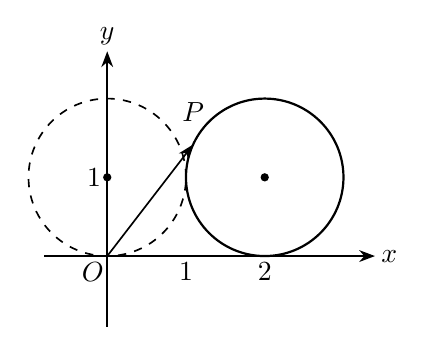
\begin{tikzpicture}[x=1cm,y=1cm,line width=.6pt,font=\normalsize,every node/.style={inner sep=0pt},>=Stealth]
\draw[->] (-0.8,0)--(3.4,0) node[right,xshift=2pt] {$x$};
\draw[->] (0,-0.9)--(0,2.6) node[above,yshift=2pt] {$y$};
\draw[dashed] (0,1) circle[radius=1cm];
\draw[line width=.8pt] (2,1) circle[radius=1cm];
\fill (0,1) circle(1.5pt);
\fill (2,1) circle(1.5pt);
\draw[->] (0,0)--(1.090702573174,1.416146836547);
\node[below left,xshift=-1pt,yshift=-2pt] at (0,0) {$O$};
\node[left,xshift=-2pt] at (0,1) {$1$};
\node[below,yshift=-2pt] at (1,0) {$1$};
\node[below,yshift=-2pt] at (2,0) {$2$};
\node[above,inner sep=0pt,yshift=8pt] at (1.090702573174,1.416146836547) {$P$};
\end{tikzpicture}
